
%%%%%%%%%%%%%%%%%%%%%%%%%%%%%%%%%%%%%%%%%%%%%%%%%%%%%%%%%%%%%%%%%%%%%%%%%%%%%%%%
%% CAPITULO
%%%%%%%%%%%%%%%%%%%%%%%%%%%%%%%%%%%%%%%%%%%%%%%%%%%%%%%%%%%%%%%%%%%%%%%%%%%%%%%%
\chapterimage{chapter_head_2.pdf} % Chapter heading image

\chapter{\textcolor{blue}{Historia do samba de gafieira}}
\index{Historia da samba de gafieira}


O samba de gafieira, como dança, descende principalmente do maxixe (dança),
que a sua vez foi gerado  pela união do  lundu, 
a polca e outras danças europeias.
Assim, misturando o maxixe com a ginga, e o ritmo de outras danças africanas, 
é que se obteve o que agora chamaríamos como o samba de gafieira ``primigênio''\footnote{
Primitivo; primordial; o primeiro da sua espécie. = PRIMÍGENO \cite{priberamprimigenio}.
} \cite[pp. 139]{perna2002samba}.


O aparecimento do samba nos salões de dança, 
foi um grande impacto para as pessoas que frequentavam estes lugares;
sendo considerado um ritmo novo e ligeiro,
que desagradou aos bailarinos de maior idade e menos ágeis \cite[pp. 3]{entrevistajuliojournalbrasil1}.
O senhor, Júlio Simões, socio da ``Kananga do Japão'' e
do ``Elite Club'', chegou a temer pelo futuro do seus empreendimentos; porem, para sorte dele, 
o samba fez muito sucesso no Elite,
e passou a ser considerado matéria indispensável para qualquer pessoa que pretendesse ser bailarino, 
compositor ou instrumentista \cite[pp. 3]{entrevistajuliojournalbrasil1}.

Pode-se estabelecer o ingresso do samba, aos salões de dança, entre os anos de 1930 e 1940 \cite[pp. 140]{perna2002samba}.
Para o ano de 1940 o samba dançado em salões, já tinha ganhado muita força;
porem, podia-se ver 3 formas diferentes de ser dançado \cite[pp. 142-143]{perna2002samba}:
\begin{itemize}
\item \textbf{Samba-canção (dança)}, que agora é um modo de dança extinto \cite[pp. 143]{perna2002samba},
\item \textbf{Samba-batucada}, que é o samba de gafieira primigênio \cite[pp. 143]{perna2002samba}, e
\item \textbf{Samba liso}, que é um estilo de dança que perdura ainda ate nossos dias \cite[pp. 143]{perna2002samba}, ver Seção \ref{subsec:estilosdedanca}.
\end{itemize}
Com o passar dos anos foram agregados elementos de outras danças a esse primitivo, samba de gafieira;
por exemplo, movimentos do tango e do rock \cite[pp. 142]{perna2002samba}.

A Figura \ref{fig:formuladosambagafieira} mostra o árvore genealógico de nosso samba de gafieira atual.
\begin{figure}[h]
  \centering
    \includegraphics[width=0.6\textwidth]{chapters/cap-historia-sambagafieira/sambagafieiraformula.eps}
  \caption{Formula da criação do samba de gafieira.}
\label{fig:formuladosambagafieira}
\end{figure}

%%%%%%%%%%%%%%%%%%%%%%%%%%%%%%%%%%%%%%%%%%%%%%%%%%%%%%%%%%%%%%%%%%%%%%%%%%%%%%%
\section{\textcolor{blue}{Em que estilos musicais posso dançar samba de gafieira?}}
\label{subsec:gafieiradancaestilos}

Entre os estilos musicais em que o samba de gafieira se adapta bem, temos:
\begin{itemize}
\item \textbf{Samba de gafieira}
\item \textbf{Samba de breque}
\item \textbf{Pagode paulista}
\item \textbf{Partido alto}
\item \textbf{Pagode carioca}
\item \textbf{Samba canção}
\item \textbf{Bossa nova}
\item \textbf{Choro}.
%\item \textbf{}
\end{itemize}

A Figura \ref{fig:gafieiradancaestilos} mostra um resumo dos 
tipos de estilos musicais onde pode ser dançado samba de gafieira.
\begin{figure}[h]
  \centering
    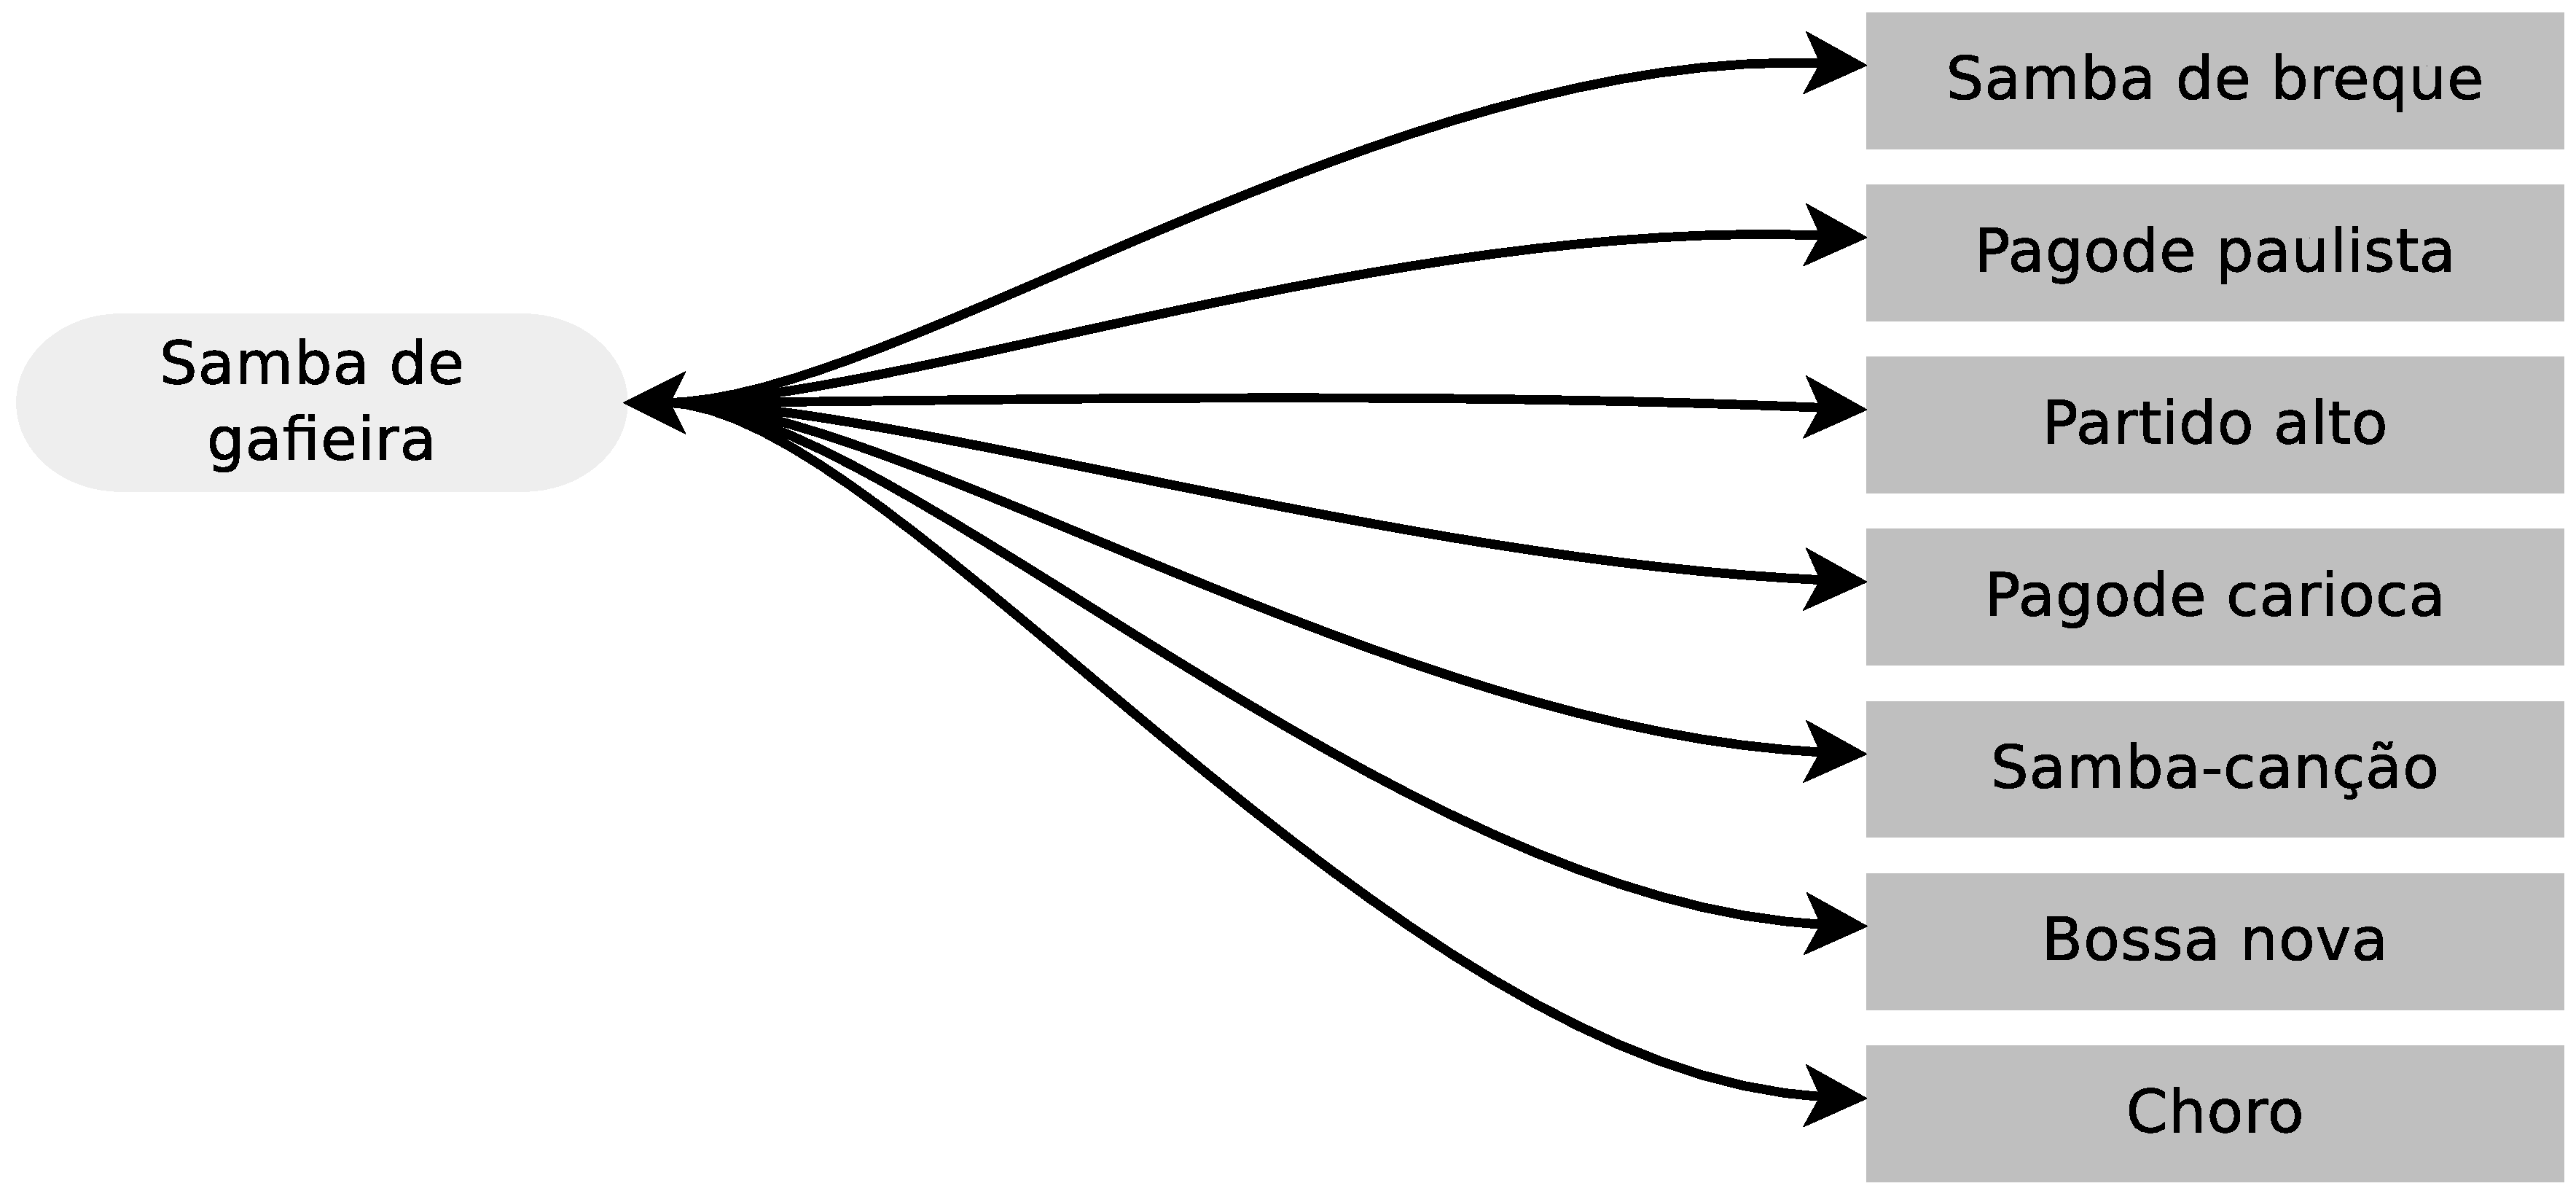
\includegraphics[width=0.6\textwidth]{chapters/cap-historia-sambagafieira/gafieiravcmusica.eps}
  \caption{ Estilos de músicas no samba onde pode-se dançar samba de gafieira.}
\label{fig:gafieiradancaestilos}
\end{figure}

%%%%%%%%%%%%%%%%%%%%%%%%%%%%%%%%%%%%%%%%%%%%%%%%%%%%%%%%%%%%%%%%%%%%%%%%%%%%%%%
\section{\textcolor{blue}{Quais são os passos de samba de gafieira?}}

Os passos do samba de gafieira primigênio são \cite[pp. 142]{perna2002samba}:
\begin{tasks}
\task \textbf{Balão}.
\task \textbf{Balão apagado}.
\task \textbf{Pica-pau}. 
\end{tasks}~\\


Em palavras de Jimmy de Oliveira os movimentos que já existiam antes do 1990 são \cite{sambafunkeadoJimmyDeOliveiraPart1}:
\begin{tasks}
\task \textbf{Picadilho} ou picadinho  
\task \textbf{Pião}
\end{tasks}~\\

Os passos criados a finais da década de 1980 e inícios de 1990 são \cite[pp. 143]{perna2002samba}:
\begin{tasks}
\task \textbf{Caminhada}, ou caminhada a contratempo.
\task \textbf{Chicote}.
\task \textbf{Esse}.
\task \textbf{Facão}.
\task \textbf{Faquinha}.
\task \textbf{Gancho}.
\task \textbf{Gancho redondo}.
\task \textbf{Letra}.
\task \textbf{Puladinho redondo}.
\task \textbf{Trança}.
\task \textbf{Tesoura}.
\end{tasks}~\\


Jimmy de Oliveira criou, apos os anos 1990 \cite{sambafunkeadoJimmyDeOliveiraPart1}: 
\begin{tasks}
\task \textbf{Assalto}. 
\task \textbf{Boneca}.
\task \textbf{Elástico}.
\task \textbf{Escovinha}.
\task \textbf{Homem vai a lua}.  
\task \textbf{Pescaria}.
\task \textbf{Romário}.
\end{tasks}~\\



Outros movimentos sem data conhecida são \cite[pp. 143]{perna2002samba}:
\begin{tasks}
\task \textbf{Bicicleta}.
\task \textbf{Cruzado}.
\task \textbf{Cadeirinha}.
\task \textbf{Puladinho}, neste movimento não se pula, lembremos que o diminutivo de pular é pulinho; 
existem varias referencias não acadêmicas na internet, que datam desde o 2002,
onde não mencionam ao ``Puladinho'' e sim um passo chamado ``pruladinho'', pelo qual suspeito que é o nome primigênio do passo;
pois indica corretamente que no movimento se vá ``pra o ladinho''.
\end{tasks}~\\


Passos acrobáticos ou para apresentações \cite[pp. 142-143]{perna2002samba}:
\begin{tasks}
\task \textbf{Cabide}, oriundo do rock.
\task \textbf{Baratinha}
\task \textbf{Enceradeira}, criado em algum momento no final da década de 1980 e inícios da década de 1990.
\end{tasks}


%%%%%%%%%%%%%%%%%%%%%%%%%%%%%%%%%%%%%%%%%%%%%%%%%%%%%%%%%%%%%%%%%%%%%%%%%%%%%%%
\section{Sobre o $syllabus$ da samba de gafieira}

O syllabus  do samba de gafieira, foi criado no ano 2001 em Rio de Janeiro,
este é um listado de passos ordenado em três níveis (iniciante, intermediário e avançado),
selecionados por votação,
onde são agrupados passos que se consideram essenciais para o ensino e competição;
neste listado não entram passos aéreos \cite[pp. 144]{perna2002samba}.


As personas que participaram da votação para a elaboração do syllabus são \cite[pp. 144]{perna2002samba}:
\begin{inparaitem}[$\circ$]
\item Carlinhos de Jesus
\item Marco Antonio Perna
\item Rogério Mendonça
\item Dani Escudero
\item Marquinhos Copacabana
\item Bob Cunha e Aurya
\item Dani Galper
\item Dani Aguiar
\item Kilve
\item Flávio Miguel
\item Bolacha
\item Luis Florião/Adriana
\item Gérson Reis
\item Egídio
\item Bruno Barros
\item Wanir Almeida
\item Valdeci
\item Marcello Moragas
\end{inparaitem}.\\



Nos passos nível básico temos:
\begin{tasks}(2)
\task Básico (frente-trás)
\task Balanço 
\task Cruzado
\task Gancho
\task puladinho
\task Esse
\task Tirada ao lado
\task Saída lateral
\task Caminhada ou caminhada a contratempo
\task Giro da dama
\end{tasks}~\\


Os passos de nível intermediário são:
\begin{tasks}(2)
\task Tirada de perna
\task Romário
\task Gancho redondo
\task Facão
\task Trança
\task Assalto
\task Tesoura
\task Balão apagado
\task Mestre sala
\task Escovinha
\end{tasks}~\\

Os passos de nível avançado são:
\begin{tasks}(2)
\task Pião
\task Picadinho ou ou picadilho
\task Bicicleta
\task Pica-pau
\task Enceradeira
\end{tasks}

